\documentclass{ctexart}
\usepackage{EC}
\begin{document}
\section{氮及其化合物}
\subsection{单质氮}
\ce{N2}几乎是氮唯一稳定的单质.
\begin{substance}[\ce{N2}]
    氮气,化学式为\ce{N2},是一种无色无味无臭的反磁性气体,熔点为$-210\tc$,沸点为$-195.8\tc$,极易溶于水.
\end{substance}
\subsubsection{\ce{N2}的化学性质}
\ce{N2}在常温下是相当不活泼的,这可能是因为
\begin{enumerate}[label=\tbf{\arabic*.},topsep=0pt,parsep=0pt,itemsep=0pt,partopsep=0pt]
    \item \ce{N2}具有很大的键能(键解离能为$945.41\kJm$).
    \item \ce{N2}的HOMO-LUMO能级间距大.
    \item \ce{N#N}键的电子分布非常均匀,没有极性.
\end{enumerate}
\ce{N2}的反应性随温度升高而增加.\ce{N2}能与活泼金属反应生成氮化物,与\ce{H2}反应\footnote{这是化工行业重要的反应之一,也常常出现于各类平衡计算中.}生成\ce{NH3},与焦炭反应生成\ce{(CN)2}:
\begin{center}
    \ce{2C + N2 ->T[$\Delta$] (CN)2}
\end{center}
虽然\ce{N2}相比\ce{CO}也是一个较差的配体,但仍然能形成各种配合物.最早制得的\ce{N2}配合物为\ce{[Ru(NH3)5(N2)]^2+},是用水合肼还原\ce{RuCl3}水溶液而制得的.\ce{N2}的配合物是无机化学研究的重要领域,这与固氮有着重要的关联.
\subsubsection{\ce{N2}的生产与用途}
大规模制取\ce{N2}的唯一途径是分馏空气(这和制取\ce{O2}是一致的),实验室也多采取氮气瓶供给的方式实现.其它的可行的办法包括:
\begin{center}
    \ce{2NaN3 ->T[$300\tc$] 2Na + 3N2}\\
    \ce{NH4NO2(aq) ->T[$\Delta$] N2(g) + 2H2O(l)}\\
    \ce{(NH4)2Cr2O7 -> N2 + 2Cr2O3 + 4H2O}\\
    \ce{8NH3 + 3Br2 ->T[aq] N2 + 6NH4Br}\\
    \ce{2NH3 + 3CuO -> N2 + 3Cu + 3H2O}
\end{center}
\subsection{全氮离子}
我们主要介绍两种全氮离子:\ce{N5+}和\ce{N5-}.巧合的是,这两种离子分别由美国和中国的研究团队发现,并且都是研发高能炸药时制得的.
\subsubsection{全氮阳离子}
\ce{N5+}唯一的制备方法如下:
\begin{center}
    \ce{cis-N2F2 + SbF5 ->T[$-78\tc$] [N2F]+[SbF6]-}\\
    \ce{ [N2F]+[SbF6]- + HN3 ->T[$-78\tc$][\ce{HF}] [N5]+[SbF6]- + HF}
\end{center}
\ce{N5+}的结构示意如下.
\chemfig{N5+}{1}{\ce{N5+}的结构}
你可以尝试画出它的共振式以验证这一结构的合理性.\\
\indent 值得一提的是,\ce{N5+}可以形成诸如\ce{[N5]+[P(N3)6]-}和\ce{[N5]+[B(N3)4]-}的离子.它们也许是含\ce{N}量较高的化合物之一.
\subsubsection{全氮阴离子}
2017年,中国南京理工大学化工学院胡炳成教授课题组首次合成出室温下稳定的\ce{N5-}盐,发表于Science杂志上.
\chemfig{N5-}{1}{\ce{N5-}的合成路线及其结构}
这一离子的稳定性部分源于其芳香性,它是咪唑阴离子的等电子体.笔者猜测\ce{HN5}也许是含\ce{N}量最高的化合物.\footnote{可惜的是,\ce{[N5]+[N5]-}理当不存在.否则我们就能见到一种看起来就很适合做炸药的物质了.}
\subsection{氮化物}
\subsubsection{氮化物}
氮几乎和周期表中的所有元素形成二元化合物(略少于\ce{O}和\ce{F}).它们的结构通常比较复杂.金属氮化物的制备方式主要有:
\begin{enumerate}[label=\tbf{\arabic*.},topsep=0pt,parsep=0pt,itemsep=0pt,partopsep=0pt]
    \item 金属与\ce{N2}(通常在高温下)反应,例如
        \begin{center}
            \ce{3Ca + N2 -> Ca3N2}
        \end{center}
    \item 金属与\ce{NH3}(通常也在高温下)反应,例如
        \begin{center}
            \ce{3Mg + 2NH3 -> Mg3N2 + 3H2}
        \end{center}
    \item 金属氨基化合物的热分解,例如
        \begin{center}
            \ce{3Zn(NH2)2 -> Zn3N2 + 4NH3}
        \end{center}
    \item 在有还原剂存在时还原金属氧化物或卤化物,例如
        \begin{center}
            \ce{Al2O3 + 3C + N2 -> 2AlN + 3CO}\\
            \ce{2ZrCl4 + N2 + 4H2 -> 2ZrN + 8HCl}
        \end{center}
    \item 在液氨中进行的反应.
\end{enumerate}
根据性质的不同,我们可以把氮化物分成三类:离子型,共价型和金属型.
\subsubsection{叠氮化物}
\subsection{氨和铵盐}
\begin{substance}[\ce{NH3}]
    氨,化学式为\ce{NH3},是无色的具有特殊刺激性气味的气体.较高浓度的\ce{NH3}是有毒的.\ce{NH3}的熔点为$-77.7\tc$,沸点为$-33.4\tc$.
\end{substance}
\subsubsection{氨的结构与物理性质}
液态\ce{NH3}具有较低的密度和粘度,但具有很高的介电常数.\\
\indent 一个有必要探讨的话题是固态氨中的氢键数目.事实上,与\ce{H2O}不同,固态氨中的每个\ce{N}原子均形成三组氢键,因此这一氢键事实上与冰中具有芳香性和饱和性的氢键并不相同,更像是一种静电相互作用.这也导致了固态氨融化时实际上沉在液相的底部\footnote{参考数据:$198\K$时,液氨的密度为$0.731\text g\cdot\text{cm}^{-3}$;$193\K$时固态氨的密度为$0.820\text g\cdot\text{cm}^{-3}$.},这与冰和水恰恰相反.
\subsubsection{液氨作为一种溶剂}
液氨是人们最熟悉的,研究得最充分的非水离子化体系.在这其中可以发生许多典型的反应.
\paragraph{溶解碱金属}
碱金属最引人注意的性质之一是它们易溶于液氮并形成亮蓝色的,具有异乎寻常性质的亚稳态溶液.重碱土金属,\ce{Eu}和\ce{Yb}也有类似的性质.\\
\indent 这些溶液具有相似的性质.在浓度较低时,它们都呈现蓝色,而在浓度较高时则显现金属般的赤褐色.随着浓度增大,溶液的电导率先减小后增大,磁性也由低浓度的顺磁性变为抗磁性,最后又显现微弱的顺磁性.\\
\indent 现在,我们普遍认为其中含有金属离子\ce{M^x+}的氨配合物\ce{[M(NH3)n]^x+}和分布在空穴中的自由电子\ce{e-}.这些空穴是排开\ce{NH3}分子形成的,因此会使得溶液密度大大减小.溶液显现蓝色正是由于自由电子的存在.\\
\indent 在Greenwood的元素化学中,这一现象是按照如下方法解释的.我们可以用以下几种物质的平衡来解释金属-液氨溶液随浓度发生的性质变化\footnote{这里省略表示了\ce{NH3}的溶剂化作用.}:
\begin{center}
    \ce{M <=> M^+ + e^-}\ \ \ $K\sim10^{-2}$\\
    \ce{M + e- <=> M-}\ \ \ $K\sim10^{-3}$\\
    \ce{2M <=> M2}\ \ \ $K\sim5\times10^{3}$
\end{center}
当\ce{M}的总浓度较低时,第一个平衡占主要地位.此时,由于自由电子\ce{e-}的存在,溶液呈现顺磁性,并且由于\ce{e-}极高的离子迁移率,溶液的摩尔电导率也较高.当\ce{M}的浓度升高时,\ce{e-}与\ce{M}结合形成\ce{M-},摩尔电导率降低,同时二聚体\ce{M2}的形成也使得溶液呈现抗磁性.\\
\indent 近年来的研究表明\footnote{E. Zurek, P.P. Edwards, R. Hoffmann, A molecular perspective on lithium-ammonia solutions, \textit{Angew. Chem. Int. Ed.} \tbf{2009}, \textit{48}, 8198-8232, https://doi.org/10.1002/anie.200900373.},按照以下模型来描述可能更好.
\begin{enumerate}[label=\tbf{\arabic*.},topsep=0pt,parsep=0pt,itemsep=0pt,partopsep=0pt]
    \item \tbf{低浓度}(大约$<10^{-3}$ mol\%)\\
        首先,碱金属溶于液氨并电离为\ce{[M(NH3)_n]^+}和氨合电子\ce{[e^-\text{@}(NH3)_m]}.随着浓度升高,阴阳离子发生明显的缔合作用.主要的缔合方式有两种:
        \begin{center}
            \ce{\ce{[M(NH3)_n]^+} + \ce{[e^-\text{@}(NH3)_m]} -> [\ce{M(NH3)_n^+}.\ce{e^-\text{@}(NH3)_m}]}\\
            \ce{\ce{[M(NH3)_n]^+} + \ce{[e^-\text{@}(NH3)_m]} -> M(NH3)_n + m NH3}
        \end{center}
        以及形成一系列聚合物种.
    \item \tbf{中等浓度}(大约$10^{-3}\sim1$ mol\%)\\
        在此阶段,除去缔合作用以外,各种顺磁性物种还会发生缔合,使得溶液的磁导率下降:
        \begin{center}
            \ce{\ce{2[e^-\text{@}(NH3)_m]} -> \ce{[(e^-)_2\text{@}(NH3)_p]}}\\
            \ce{2 M(NH3)_n -> M2(NH3)_q}
        \end{center}
        也许\ce{M2(NH3)_q}写作\ce{\{[M(NH3)_n]^+_2.\ce{(2e^-)\text{@}(NH3)_m}\}}比较合适.\\
        直至大约$0.5\sim1$ mol\%时,溶液中几乎所有顺磁性物种(主要是氨合电子)都发生自旋配对,溶液呈现抗磁性.
    \item \tbf{高浓度}(大约$>4$ mol\%)\\
        溶液发生向金属态的转变(Transition to the Metallic State, TMS).溶液的摩尔电导率迅速上升,直至和液态金属相当,同时呈现微弱的顺磁性.自然,颜色也由蓝色变为典型的青铜色.研究认为,此时溶液主要以聚合物为主.典型的聚合物有下面几种.
        \begin{center}
            \ce{[\ce{M(NH3)_n^+}.\ce{e^-\text{@}(NH3)_m}]_r}\\
            \ce{[\ce{M(NH3)_n}.\ce{e^-\text{@}(NH3)_m}]_r}\\
            \ce{[M(NH3)_n]_r}
        \end{center}
\end{enumerate} 
\indent 碱金属的液氨溶液不稳定.在有杂质作为催化剂或放置的较久的情况下,这些溶液将分解为对应的氨基盐:
\begin{center}
    \ce{2Na + 2NH3 -> 2NaNH2 v + H2}
\end{center}
需要注意的是,\ce{NaNH2}微溶于液氨,因此放置的太久的\ce{Na}-\ce{NH3}溶液发生的现象为:溶液的蓝色逐渐褪去,产生白色沉淀.\\
\indent 由碱金属-液氨溶液出发也可以获得以电子作为阴离子的盐.例如:
\begin{center}
    \ce{Na + 2,2,2-crypt ->T[\ce{NH3(l)}][vap] [Na(2,2,2-crypt)]^+e^-}
\end{center}
所得的\ce{[Na(2,2,2-crypt)]^+e^-}是一种蓝黑色的顺磁性物质.\\
\indent 碱金属的液氨溶液具有很强的还原性.并且,由于这还原性是自由电子\ce{e-}体现的,因此它常常能做到对物质的单电子还原.例如:
\begin{center}
    \ce{Mn2(CO)10 + 2K ->T[\ce{NH3(l)}] 2K[Mn(CO)5]}\\
    \ce{Fe(CO)5 + 2Na ->T[\ce{NH3(l)}] Na2[Fe(CO)4] + CO}
\end{center}
等等.碱金属的液氨溶液在有机化学中也被广泛地运用于还原各种物质,例如将炔烃还原为反式烯烃,Birch还原等等.
\paragraph{液氨中的复分解反应}
大部分时候,我们可以把液氨中的反应与水溶液中的反应进行类比.然而,由于结构与性质上的差异,许多物质在水中的溶解度和在液氨中有明显的不同.典型的微溶物有\ce{NaF},\ce{NaCl}.大多数铵盐都易溶,而\ce{AgBr}等物质由于可以形成\ce{Ag(NH3)2+}配离子,也是易溶的.这就造成了某些水溶液中不能进行的反应反而能在液氨中进行:
\begin{center}
    \ce{Ba(NO3)2 + 2AgBr ->T[\ce{NH3(l)}] BaBr2 v + 2AgNO3}
\end{center}
以及与难氢氧化物和氧化物的形成类似地有
\begin{center}
    \ce{AgNO3 + KNH2 ->T[\ce{NH3(l)}] AgNH2 v + KNO3}\\
    \ce{3HgI2 + 6KNH2 ->T[\ce{NH3(l)}] Hg3N2 + 6KI + 4NH3}
\end{center}
\paragraph{液氨中的酸碱反应}
和水一样,液氨也可以发生自耦电离:
\begin{center}
    \ce{2NH3 <=> NH4+ + NH2-}\ \ \ $K=1.9\times10^{-33}$
\end{center}
因此体系中可以发生与水溶液中类似的酸碱反应.此外,还有一些物质具有两性:
\begin{center}
    \ce{K2[Zn(NH2)4] + 2NH4NO3 ->T[\ce{NH3(l)}] Zn(NH2)2 + 2KNO3 + 4NH3}\\
    \ce{Zn(NH2)2 + 2NH4NO3 ->T[\ce{NH3(l)}] [Zn(NH3)4](NO3)2}
\end{center}
\paragraph{液氨中的氧化还原反应}
理论分析表明,不考虑动力学因素时,液氨中不会有比\ce{N2}更强的氧化剂,也不会有比\ce{H2}更强的还原剂.这仅仅对应于$0.04\V$的电位区间.不过由于超电势的存在,实际的范围要大得多.不过,仍然会发生缓慢的反应.例如,\ce{NO3-}在碱性溶液中放出\ce{N2}:
\begin{center}
    \ce{3K+ + 3NH2- + 3NO3- ->T[\ce{NH3(l)}] 3KOH v + N2 + 3NO2- + NH3}
\end{center}
\subsubsection{氨的化学性质}
\ce{NH3}溶于水即生成一水合氨.在水中,\ce{NH3}是弱碱:
\begin{center}
    \ce{NH3(aq) + H2O(l) <=> NH4+(aq) + OH-(aq)}\ \ \ $K=1.81\times10^{-5}$
\end{center}

\indent 氨在空气中很难燃烧,但在催化剂的存在下可以被选择性地氧化为\ce{NO}.\ce{NO}接着可以被氧化为\ce{NO2},这也是工业制\ce{HNO3}的方法:
\begin{center}
    \ce{4NH3 + 3O2 ->T[点燃] 2N2 + 6H2O}\\
    \ce{4Nh3 + 5O2 ->T[\ce{Pt}][$800\tc$] 4NO + 6H2O}
\end{center}
此外,利用Andrussow法工业生产\ce{HCN}也存在\ce{NH3}的氧化.\\
\indent \ce{NH3}在\ce{F2}中燃烧,形成黄绿色火焰,生成\ce{NF3}.\ce{NH3}在\ce{Cl2}中的燃烧则复杂得多.不过,在正常条件下可以发生反应
\begin{center}
    \ce{8NH3 + 3Cl2 -> 6NH4Cl + N2}
\end{center}
这一反应可以用于检测\ce{Cl2}管道的泄漏.由于\ce{NH4Cl}为白色固体,因此有\ce{Cl2}存在的地方会产生明显的白烟.\\
\indent 需要特别注意的是,由于\ce{Cu}离子与\ce{NH3}具有很好的络合作用,因此有\ce{O2}存在时\ce{NH3}将迅速地侵蚀\ce{Cu}单质.因此,不能用含\ce{Cu}的管道材料运输\ce{NH3}.
\subsubsection{氨的合成}
请自行查阅合成氨的相关内容.
\subsection{氮的其它氢化物}
除\ce{NH3}和五唑\ce{HN5}以外,氮还可以与氢形成联氨\ce{N2H4},叠氮酸\ce{HN3}等等氢化物.
\subsubsection{联氨\ce{N2H4}}
\begin{substance}[\ce{N2H4}]
    联氨,化学式为\ce{N2H4}.无水联氨为无色发烟液体,熔点$2.0\tc$,沸点$113.5\tc$.
\end{substance}
联氨和水的物理性质在很多方面上都比较相似.
\paragraph{联氨的结构}
气相中的联氨呈现歪扭式的结构.
\paragraph{联氨的碱性}
由于\ce{N}的吸电子效应,\ce{N2H4}在水溶液中的碱性弱于\ce{NH3}:
\begin{center}
    \ce{N2H4(aq) + H2O(l) <=> N2H5+(aq) + OH-(aq)}\ \ \ $K_{\text b1}=8.5\times10^{-7}$\\
    \ce{N2H5+(aq) + H2O(l) <=> N2H6^2+(aq) + OH-(aq)}\ \ \ $K_{\text b1}=8.9\times10^{-16}$
\end{center}
\paragraph{联氨的制备与反应}
一般可以通过下面的方法制备\ce{N2H4}:
\begin{center}
    \ce{2NH3 + NaOCl ->T[强碱水溶液] N2H4 + NaCl + H2O}
\end{center}
这一反应可能的机理如下:
\begin{center}
    \ce{NH3 + ClO- -> NH2Cl + OH-}\\
    \ce{NH3 + NH2Cl -> N2H5+ + Cl-}\\
    \ce{N2H5+ + OH- -> N2H4 + H2O}
\end{center}
联氨可以通过如下方式被滴定:
\begin{center}
    \ce{N2H4 + KIO3 + 2HCl ->T[\ce{H2O}/\ce{CCl4}] N2 + KCl + ICl + 3H2O}
\end{center}
以\ce{KIO3}作为滴定剂,反应首先生成\ce{I2}使得\ce{CCl4}相变为紫色,然后继续加入\ce{KIO3}又将其氧化为\ce{ICl},利用\ce{CCl4}相中\ce{I2}颜色的完全消失判断终点.
\subsubsection{羟胺\ce{NH2OH}}
由于羟胺的性质与联氨有一定相似之处,因此放在氢化物一节一同介绍.
\begin{substance}[\ce{NH2OH}]
    羟胺,化学式为\ce{NH2OH}.无水羟胺为无色,对热不稳定的白色固体,熔点$33\tc$,沸点$110\tc$.
\end{substance}
\paragraph{羟胺的结构}
\ce{NH2OH}的结构在在不同情况下差异较大.在晶体中,\ce{NH2OH}倾向于以反式的构象.
\paragraph{羟胺的碱性}
羟胺的碱性比\ce{N2H4}或\ce{NH3}都要弱:
\begin{center}
    \ce{NH2OH(aq) + H2O(l) <=> NH3OH+(aq) + OH-(aq)}\ \ \ $K_\text b=6.6\times10^{-9}$
\end{center}
\paragraph{羟胺的制备与反应}
\ce{NH2OH}可以通过许多反应制得.例如Raschig法合成\ce{NH2OH}:
\begin{center}
    \ce{NH4NO2 + 2SO2 + NH3 + H2O -> (NH4)2[N(OH)(OSO2)2]}\\
    \ce{(NH4)2[N(OH)(OSO2)2] + 2H2O -> NH2OH + 2NH4HSO4}
\end{center}
或者利用下面几种方法制备羟胺盐:
\begin{center}
    \ce{2NO(g) + 3H2(g) + H2SO4(aq) ->T[\ce{Pt/C}]} (NH3OH)2SO4\\
    \ce{2RCH2NO2 + 2H2O + H2SO4 -> 2RCOOH + (NH3OH)2SO4}\\
    \ce{C2H4 + 2NO2 -> O2NCH2CH2NO2}\ \ \ \ \ \ce{O2NCH2CH2NO2 + H2SO4 -> CO2 + CO + (NH3OH)2SO4}
\end{center}
实验室中常用\ce{HSO3-}还原\ce{HNO2}制备,这与Raschig法类似.
\subsubsection{叠氮酸\ce{HN3}及其盐}
\begin{substance}[\ce{HN3}]
    叠氮酸,化学式为\ce{HN3},是一种具有令人厌恶的刺激性气味的液体或气体,熔点$-80\tc$.\ce{HN3}具有强烈的爆炸性,并且是一种剧毒的物质.
\end{substance}
\begin{substance}[\ce{NaN3}]
    叠氮化钠,化学式为\ce{NaN3},是一种剧毒且易爆的白色固体,加热至$275\tc$时分解.
\end{substance}
\paragraph{\ce{HN3}与\ce{N3-}的结构}
气相中的\ce{HN3}为折线形分子,\ce{N}原子在同一直线上,\ce{HN-N2}键长$124\text{ pm}$,\ce{HN2-N}键长$113\text{ pm}$.键角为$112^\circ$.\\
\indent \ce{N3-}作为\ce{CO2}的等电子体,是直线型离子,其中\ce{N-N}键键长均为$116\text{ pm}$.
\paragraph{\ce{HN3}的酸性}
\ce{HN3}在水溶液中为弱酸,酸性与醋酸比较接近:
\begin{center}
    \ce{HN3(aq) + H2O(aq) -> H3O+(aq) + N3-(aq)}\ \ \ $K_\text a=1.8\times10^5$,$\text pK_\text a=4.77$
\end{center}
\paragraph{\ce{HN3}与\ce{N3-}的制备与性质}
叠氮酸最早被通过以下方法制得:
\begin{center}
    \ce{N2H5+ + HNO2 -> HN3 + H+ +2H2O}
\end{center}
不过通常可以通过小心酸化\ce{NaN3}的方式制备.大多数制取叠氮酸及其衍生物的方法都要用到\ce{NaN3},它可以通过如下方式制备:
\begin{center}
    \ce{NaNO2 + 3NaNH2 ->T[熔融] NaN3 + 3NaOH + NH3}\\
    \ce{N2O + 2NaNH2 ->T[熔融] NaN3 + NaOH + NH3}(在\ce{NH3(l)}中进行反应亦可)\\
    \ce{3N2O + 4Na + NH3 -> NaN3 + 3NaOH + 2N2}
\end{center}
叠氮化物的主要用途取决于其爆炸性.例如,汽车安全气囊中曾经就置有\ce{NaN3},分解时放出大量\ce{N2}充满气囊,起到缓冲作用:
\begin{center}
    \ce{2NaN3 -> 2Na + 3N2}
\end{center}
而\ce{Pb(NO3)2}与\ce{NaN3}的复分解反应的产物\ce{Pb(N3)2}则由于其可靠性(尤其是在潮湿环境中)而被广泛地用作引爆剂.
\subsubsection{二亚胺\ce{N2H2}}
笔者几乎只在有机化学上见过这一物质.顺式的二亚胺可以用作还原剂对烯烃进行顺式加氢,同时生成\ce{N2}.
\subsection{氮的卤化物与卤氧化物}
1811年,P.L.Dulong历经千辛万苦制得了\ce{NCl3}(他为此付出了三根手指和一只眼睛的代价).令人费解的是\ce{N}最稳定的卤化物\ce{NF3}直到115年后才被制得.
\subsubsection{氮的氟化物}
\paragraph{\ce{NF3}}
纯的\ce{NF3}首先是利用电解\ce{NH4F/HF}熔融物而制备的;另一个可用的方法是在\ce{Cu}催化剂上对\ce{NH3}进行控制氟化:
\begin{center}
    \ce{NH4F + 2HF ->T[熔融][电解] NF3 + 3H2}\\
    \ce{4NH3 + 3F2 ->T[\ce{Cu}] NF3 + 3NH4F}
\end{center}
\begin{substance}[\ce{NF3}]
    三氟化氮,化学式为\ce{NF3},是无色无臭的稳定气体,熔点为$-206.8\tc$,沸点为$-129.0\tc$.
\end{substance}
\indent\ce{NF3}分子为三角锥形,键角为$102.5^\circ$,偶极矩异常地小(仅为\ce{NH3}的六分之一).这是由于\ce{N-F}键矩方向与孤对电子方向相反所致.\\
\indent 在常温下,\ce{NF3}是不活泼的.升高温度时\ce{NF3}可以作为氟化剂:
\begin{center}
    \ce{2NF3 + 2Cu -> N2F4 + CuF2}
\end{center}
尽管\ce{NF3}是稳定的,但它仍然能形成一些四面体构型的离子:
\begin{center}
    \ce{NF3 + F2 + SbF5 ->T[$200\tc$][100 atm][NF4]+[SbF6]-}\\
    \ce{2NF3 + O2 ->T[放电][$-196\tc$] 2ONF3}\\
    \ce{3NOF + 2IrF6 ->T[$20\tc$] ONF3 + 2[NO]+[IrF6]-}
\end{center}
\ce{NOF3}中有着明显短的\ce{N-O}键(115.8 pm)和明显长的\ce{N-F}键(143.1 pm).
\paragraph{\ce{N2F4}}
\ce{N2F4}除了用\ce{Cu}还原\ce{NF3}得到外还可以通过以下方式得到:
\begin{center}
    \ce{CO(NH2)2 + 2F2 ->T[\ce{N2/F2}] H2NCONF2 + 2HF}\\
    \ce{NH2CONF2 ->T[浓\ce{H2SO4}] NF2H + HOCN}\\
    \ce{2NF2H + NaOCl -> N2F4 + H2O + NaCl}
\end{center}
\begin{substance}[\ce{N2F4}]
    四氟化二氮,化学式为\ce{N2F4},是无色气体,熔点为$-164.5\tc$,沸点为$-73\tc$.
\end{substance}
\indent\ce{N2F4}是较为活泼的气体,可以作为氟化剂与很多物质发生反应,例如:
\begin{center}
    \ce{10Li + N2F4 -> 4LiF + 2Li3N}
\end{center}
此外,\ce{N2F4}还能离解产生\ce{F2N.}自由基.在低压下快速冷冻\ce{N2F4}就能得到暗蓝色的固体.事实上,\ce{N2F4}的很多化学性质也与\ce{F2N.}自由基有关,例如:
\begin{center}
    \ce{N2F4 + 2PhSH -> PhSSPh + 2NF2H}\\
    \ce{N2F4 + 2NO -> 2F2NNO}
\end{center}
\paragraph{\ce{N2F2}}最好的制备\ce{N2F2}的方法如下:
\begin{center}
    KF + NF2H ->T[$-80\tc$][then $20\tc$] KHF2 + N2F2
\end{center}
制得的\ce{N2F2}一般是顺式和反式异构体的混合物.
\begin{substance}[\ce{N2F2}]
    二氟化二氮,化学式为\ce{N2F2},是无色气体.\\
    cis-\ce{N2F2}的熔点低于$-195\tc$,沸点为$-105.7\tc$;trans-\ce{N2F2}的熔点为$-172\tc$,沸点为$-111.4\tc$.
\end{substance}
下面是两种异构体的键长数据.
\begin{table}[H]
    \centering
    \begin{tabular}{|c|c|c|}
        \hline
        键长/pm&\ce{N=N}&\ce{N-F}\\\hline
        顺式\ce{N2F2}&120.9&140.9\\\hline
        反式\ce{N2F2}&122.4&139.8\\\hline
    \end{tabular}
\end{table}
造成键长差异的原因主要是\ce{N}的孤对电子对$\sigma^\ast\left(\ce{N-F}\right)$轨道的超共轭作用,这一作用削弱\ce{N-F}键而加强\ce{N=N}键,也为分子提供了额外的稳定化作用.因此,顺式\ce{N2F2}在热力学上更加稳定,在气相的平衡中也占据主要.\\
\indent 然而,顺式\ce{N2F2}在动力学上似乎更加活泼.顺式\ce{N2F2}在玻璃容器内存放两周即完全反应:
\begin{center}
    \ce{SiO2 + 2N2F2 -> SiF4 + 2N2O}
\end{center}
反式\ce{N2F2}则可以稳定存放在玻璃容器中.此外,只有顺式\ce{N2F2}能脱去\ce{F-}形成\ce{N2F+}离子.这也是\ce{AsF5}分离两者的原理.
\subsubsection{氮的其余卤化物}
\paragraph{\ce{NCl3}}
除去氟化物外,\ce{NCl3}几乎是氮唯一稳定的卤化物.
\begin{substance}[\ce{NCl3}]
    三氯化氮,化学式为\ce{NCl3},是黄色油状液体,熔点$-40\tc$,沸点$70\tc$.
\end{substance}
\indent\ce{NCl3}可以通过电解酸性\ce{NH4Cl}溶液制得.它主要用于漂白与杀菌.\ce{NCl3}容易水解:
\begin{center}
    \ce{NCl3 + 3H2O -> NH3 + 3HOCl}\\
\end{center}
在碱性溶液中可以与\ce{NaClO2}反应制取\ce{ClO2}:
\begin{center}
    \ce{NCl3 + 3H2O + 6NaClO2 -> 6ClO2 + 3NaCl + 3NaOH + NH3}\\
    \ce{2NCl3 + 6NaClO2 -> 6ClO2 + 6NaCl + N2}
\end{center}
\paragraph{\ce{NBr3}和\ce{NI3}}
这两种化合物都十分的不稳定.
\subsubsection{氮的卤氧化物}
\paragraph{亚硝酰卤化物\ce{NOX}}
亚硝酰卤化物都是活泼气体.它们的物理性质和结构可列举如下:
\begin{table}[H]\centering
    \begin{tabular}{cccc}
        \hline
        性质    &\ce{NOF}   &\ce{NOCl}  &\ce{NOBr} \\\hline
        颜色    &无色       &橙黄色     &红色 \\
        熔点/$\tc$  &$-132.5$   &$-59.6$    &$-56$ \\
        沸点/$\tc$  &$-59.9$   &$6.4$    &$\sim0$ \\
        键角    &$110^\circ$    &$113^\circ$    &$117^\circ$\\
        \ce{N=O}键长/pm &$113$  &$114$  &$115$\\\hline
    \end{tabular}
\end{table}
它们可以通过以下方法制备:
\begin{center}
    \ce{2NO + X2 -> 2NOX}\ \ \ \ce{X=F,Cl,Br}\\
    \ce{NO + AgF2 -> NOF + Ag}\\
    \ce{N2O4 + KCl -> NOCl + KNO3}
\end{center}
\ce{NOX}在\ce{X-}受体的存在下可以裂解产生\ce{NO+},例如
\begin{center}
    \ce{NOF + BF3 -> [NO]+[BF4]-}\\
    \ce{NOCl + AlCl3 -> [NO]+[AlCl4]-}
\end{center}
\paragraph{硝酰卤化物\ce{NO2X}}
硝酰氟化物和氯化物\ce{XNO2},如同它的亚硝酰类似物,也是活泼气体;它们皆为平而形,和等电子的硝酸根\ce{NO3-}类似.它们的物理性质列举如下.
\begin{table}[H]\centering
    \begin{tabular}{ccc}
        \hline
        性质    &\ce{NO2F}   &\ce{NO2Cl} \\\hline
        熔点/$\tc$  &$-166$   &$-145$ \\
        沸点/$\tc$  &$-72.5$   &$-15.9$ \\
        \ce{X-N-O}键角    &$118^\circ$    &$115^\circ$ \\
        \ce{N-O}键长/pm &$123$  &$120$ \\\hline
    \end{tabular}
\end{table}
\ce{XNO2}的反应常常与\ce{XNO}类似.例如形成\ce{NO2+}的盐:
\begin{center}
    \ce{NO2F + BF3 -> [NO2]+[BF4]-}\\
    \ce{NO2Cl + SbCl5 -> [NO2]+[SbCl6]-}
\end{center}
\ce{NO2Cl}在水和液氨中的溶剂解也生成不同的产物.
\begin{center}
    \ce{ClNO2 + H2O -> HNO3 + HCl}\\
    \ce{ClNO2 + 2NH3 -> ClNH2 + NH4NO2}
\end{center}
造成这一差异的原因是在水中\ce{HNO2}会被\ce{HClO}氧化,而在液氨中则不发生类似的反应.
\subsection{氮的氧化物}
在众多的元素中间,氮是唯一的能形成多达(至少)7种氧化物分子的元素.所有的氮的氧化物在热力学上都是不稳定的,可分解为\ce{N2}和\ce{O2}.
\subsubsection{\ce{N2O}}
\begin{substance}[\ce{N2O}]
    一氧化二氮,俗称笑气,化学式为\ce{N2O},是无色有甜味的气体.\ce{N2O}的熔点为$-90.86\tc$,沸点为$-88.48\tc$,可以少量地溶于水中.
\end{substance}
\paragraph{\ce{N2O}的结构}
作为\ce{CO2}的等电子体,\ce{N2O}是直线型分子.理论计算表明其中\ce{N=N}键级为$2.73$,\ce{N-O}键级为$1.61$.
\paragraph{\ce{N2O}的制备}
小心地加热熔融的\ce{NH4NO3}可以使其热分解得到\ce{N2O}:
\begin{center}
    \ce{NH4NO3 ->T[$\Delta$] N2O + 2H2O}
\end{center}
这个反应的历程比较复杂.此外还有可以采用的方法为
\begin{center}
    \ce{HNO2 + NH2OH ->T[aq] N2O + 2H2O}\\
    \ce{HNO3 + HN3 ->T[aq] N2O + N2 + H2O}\\
    \ce{H2NNO2 ->T[$\Delta$] N2O + H2O}\ \ \ \ \ \ce{H2N2O2 ->T[$\Delta$] N2O + H2O}
\end{center}
尽管加热连二次硝酸\ce{H2N2O2}确实可以使其脱水得到\ce{N2O},但我们仍然不认为\ce{N2O}是连二次硝酸酐,因为\ce{N2O}溶于水并不能再次形成\ce{H2N2O2}.
\paragraph{\ce{N2O}的化学性质与反应}
室温下\ce{N2O}较不活泼,例如它不能和卤素,碱金属甚至臭
氧反应.在较高温度时它可以作为氧化剂氧化一些物质,同时生成\ce{N2}.\\
\indent \ce{N2O}的一个重要应用是制备叠氮化物.我们已经在前面介绍过.\\
\indent \ce{N2O}最大的工业应用是作为火箭推进剂和搅打起泡冰激淋(或奶油)的充气剂,这是依靠在压力下\ce{N2O}在植物油中的溶解度,以及它在低浓度时无毒无味.\ce{N2O}也大量用作麻醉剂.\\
\indent \ce{N2O}得名为笑气是因为吸入它使人欢欣并且发笑.然而,过量吸入\ce{N2O}会导致神志不清,对神经系统造成危害\footnote{\ce{N2O}能不可逆地氧化钴胺素的钴核并使甲基钴胺素失活,间接诱发维生素B12缺乏,造成神经损伤.},同时有一定的成瘾性.因此,\ce{N2O}在我国被列入《危险化学品目录》,其销售和购买需要严格监管.\\
\indent 此外,\ce{N2O}也是一种温室气体.
\subsubsection{\ce{NO}与\ce{N2O2}}
\begin{substance}[\ce{NO}]
    一氧化氮,化学式为\ce{NO},是无色无味气体,熔点为$-164\tc$,沸点为$-152\tc$.
\end{substance}
\paragraph{\ce{NO}的结构}
作为最简单的具有单电子的分子,人们对\ce{NO}的电子结构进行了详细的研究,这也推动了分子轨道理论的发展.
\paragraph{\ce{NO}的制备}
在工业上,\ce{NO}是由\ce{NH3}的催化氧化得到的,这在前面已经有所提及.\\
\indent 实验室中制取\ce{NO}可以通过以下几种方式:
\begin{center}
    \ce{2KNO2 + 2KI + 2H2SO4 -> 2NO + 2K2SO4 + H2O + I2}\\
    \ce{KNO2 + K4[Fe(CN)6] + 2CH3COOH -> NO + Ke[De(CN)6] H2O + 2CH3COOK}\\
    \ce{6NaNO2 + 3H2SO4 -> 4NO + 2HNO3 + 2H2O + 3Na2SO4}\\
    \ce{3KNO2 + KNO3 + Cr2O3 -> 4NO + 2K2CrO4}
\end{center}
\paragraph{\ce{NO}的二聚形成\ce{N2O2}}
正常情况下,\ce{NO}可以少量地二聚形成\ce{O=N-N=O}分子(先前也有人认为二聚体是矩形环状结构的,不过这被晶体的衍射数据所否定).\\
\indent 在极性物质或Lewis酸存在时冷凝\ce{NO},则可以得到红色的不对称二聚体\ce{O=N-O=N}.
\paragraph{\ce{NO}的化学性质}
\ce{NO}具有较为活泼的化学性质.\\
\indent 首先,\ce{NO}易被\ce{O2}氧化为\ce{NO2}:
\begin{center}
    \ce{2NO + O2 -> 2NO2}
\end{center}
在空气中的\ce{NO}会很快地被氧化为\ce{NO2},从而显现红棕色.这一反应还有一个有趣之处在于它是三级反应,并且表观活化能为负值.这意味着温度的升高会使得反应速率减慢.事实上,这一反应的机理如下:
\begin{center}
    \ce{2NO <=>T[$K$][快速平衡] N2O2}\\
    \ce{N2O2 + O2 ->T[$k$][慢反应] 2NO2}
\end{center}
因此反应的速率方程为$v=Kk\con{NO}^2\con{O2}$.当温度升高时,$K$减小的程度比$k$增加的程度更大,因此反应的总体速率呈现下降趋势.\\
\indent 前面已经提到过,\ce{NO}容易与卤素反应生成对应的亚硝酰卤化物.\\
\indent 鉴于\ce{NO}并没有对应价态的稳定阴离子,因此\ce{NO}在碱性条件下容易发生歧化反应:
\begin{center}
    \ce{2Na2O + 4NO ->T[$100\tc$] 2NaNO2 + Na2N2O2}\\
    \ce{2MOH + 4NO -> 2MNO2 + N2O + H2O}\\
    \ce{4MOH + 6NO -> 4MNO2 + N2 + 2H2O}
\end{center}
\paragraph{\ce{NO}的配合物}
\ce{NO}易和许多过渡金属化合物反应形成亚硝酰配合物,而且在其他的含有氧-氮物种的反应中也经常形成这类配合物.经典的例子是检验\ce{NO3-}或\ce{NO2-}棕色环实验:
\begin{center}
    \ce{3[Fe(H2O)6]^2+ + NO3- + 4H+ -> 2[Fe(H2O)6]^3+ + [Fe(H2O)5(NO)]^2+ + 3H2O}\\
    \ce{2[Fe(H2O)6]^2+ + NO2- + 2H+ -> [Fe(H2O)6]^3+ + [Fe(H2O)5(NO)]^2+ + 2H2O}
\end{center}
取待测溶液于试管中,加入适量\ce{FeSO4}溶液.缓慢沿管壁加入浓硫酸.如果在浓硫酸与溶液的界面观察到了棕色环,说明溶液中含有\ce{NO3-}或\ce{NO2-}.使用醋酸代替浓硫酸,则\ce{NO3-}不发生此反应,而\ce{NO2-}则正常.\\
\indent 通常而言,\ce{NO}在配合物中有多样的几何构型.直线型通常意味着\ce{NO}以\ce{NO+}的形式配位,作为三电子配体\footnote{形式上可以这么认为,但实际上电荷分布并非如此,\ce{NO}是通过轨道作用提供三个电子的,并非预先发生了氧化还原反应,否则会导致中心金属元素的异常低价态.}.折线形通常意味着\ce{NO}以\ce{NO-}的形式配位,作为单电子供体.\\
\indent 由于上述原因,并且\ce{NO+}与\ce{CO}为等电子体,因此简单羰基化合物中的三个\ce{CO}可以替换为两个\ce{NO}.例如
\begin{center}
    \ce{Fe(CO)5 + 2NO -> Fe(NO)2(CO)2 + 3CO}\\
    \ce{Cr(CO)6 + 4NO -> Cr(NO)4 + 6CO}
\end{center}
其它\ce{NO}的配合物将在以后提及.
\subsubsection{\ce{N2O3}}
\begin{substance}[\ce{N2O3}]
    三氧化二氮,化学式为\ce{N2O3},是一种浅蓝色固体,熔点为$-100.1\tc$,熔化后为深蓝色液体.\ce{N2O3}对热不稳定,容易分解为\ce{NO}和\ce{NO2}.
\end{substance}
\paragraph{\ce{N2O3}的结构}
\ce{N2O3}中有着异常长的\ce{N-N}键.这暗示了它离解为两种自由基\ce{NO}和\ce{NO2}的明显趋势.
\paragraph{\ce{N2O3}的化学性质}
前面已经说到\ce{N2O3}很容易分解.随着温度的升高,混合物将变为绿色(由\ce{NO2}的红棕色和\ce{N2O3}的蓝色混合而成).早先的研究总是认为\ce{NO}的液体或固体是淡蓝色的,但事实上这也是由于其中混有的少量\ce{N2O3}所显现的强烈的蓝色所致.\\
\indent 制取\ce{N2O3}的最佳方法是冷凝\ce{NO}和\ce{NO2}的等比例混合物.向\ce{NO}中混入预定比例的\ce{O2}以就地合成\ce{NO2}也是一个可采取的方法.\\
\indent 作为亚硝酸盐的酸酐,\ce{N2O3}和水反应生成\ce{HNO2},而与碱反应几乎定量地生成\ce{NO2-}.此外,在足够浓的酸中,它也可以被转化为\ce{NO+}:
\begin{center}
    \ce{N2O3 + 3H2SO4(conc) -> 2[NO]+[HSO4]- + [H3O]+[HSO4]-}
\end{center}
\subsubsection{\ce{NO2}与\ce{N2O4}}
虽然大多数时候,分别测定平衡混合物中各物质的状态是可行的,但由于\ce{NO2}与\ce{N2O4}处于极为快速的平衡中,因此大多数时候我们描述的都是平衡混合物的性质.
\begin{substance}[\ce{NO2}]
    二氧化氮,化学式为\ce{NO2},为红棕色气体,凝固点为$-11.2\tc$,沸点为$21.5\tc$.固态和液态的\ce{NO2}中实际上几乎全部为无色的\ce{N2O4}.
\end{substance}
\paragraph{\ce{NO2}和\ce{N2O4}的结构}
相比\ce{NO},\ce{NO2}中的单电子更偏向于定域在\ce{N}原子上(即SOMO轨道为\ce{N}的$\text{sp}^2$轨道).因此,\ce{NO2}发生二聚作用相对更容易一些.\\
\indent 二聚体\ce{N2O4}为平面型结构,其中的\ce{N-N}键也格外的长.
\paragraph{\ce{NO2}和\ce{N2O4}的制备}
制备\ce{NO2}最好的办法是将\ce{Pb(NO3)2}热分解的产物分级蒸馏后得到:
\begin{center}
    \ce{2Pb(NO3)2 ->T[$400\tc$] 2PbO + 4NO2 + O2}
\end{center}
其它的办法(相较而言不佳)有:
\begin{center}
    \ce{2HNO3 + SO2 -> N2O4 + H2SO4}\\
    \ce{4HNO3 + P4O10 -> 2N2O4 + O2 + 4HPO3}\\
    \ce{NOCl + AgNO3 -> N2O4 + AgCl}
\end{center}
可以看出上面的反应都可以看做先得到\ce{N2O5},再分解生成\ce{N2O4}.
\paragraph{\ce{N2O4}作为溶剂}
\ce{N2O4}作为一种优良的非水溶剂得到了大量而广泛的研究.它的独特应用是制备各种金属的无水硝酸盐.\\
\indent 在极性物质存在的形况下,\ce{N2O4}倾向于按照以下的方式解离:
\begin{center}
    \ce{N2O4 <=> NO+ + NO3-}
\end{center}
这一溶剂体系内也可以发生类似于酸碱反应的反应:
\begin{center}
    \ce{NOCl + AgNO3 -> AgCl + N2O4}\\
    \ce{2NOCl + Sn -> SnCl2 + 2NO}\\
    \ce{2EtNH3NO3 + 2N2O4 + Zn -> [EtNH3]2[Zn(NO3)4] + 2NO}\\
    \ce{CaO + 2N2O4 -> Ca(NO3)2 + N2O3}
\end{center}
这类反应为制取无水硝酸盐提供了一个很好的办法.特别是当使用金属的碘化物时,由于\ce{NOI}迅速分解,因此减少了副反应的发生,例如
\begin{center}
    \ce{TiI4 + 4N2O4 -> Ti(NO3)4 + 4NO + 2I2}
\end{center}
\indent 与\ce{N2O4}倾向于裂解为\ce{NO+}和\ce{NO3-}相比,裂解为\ce{NO2+}和\ce{NO2-}的情形则要少得多.不过,\ce{N2O4}与\ce{BF3}反应可以生成下面两种加合物:
\begin{center}
    \ce{N2O4 + BF3 -> [NO2]+[ONOBF3]-}\\
    \ce{N2O4 + 2BF3 -> [NO2]+[F3BONOBF3]-}
\end{center}
\subsubsection{\ce{N2O5}}
\begin{substance}[\ce{N2O5}]
    五氧化二氮,化学式为\ce{N2O5},是无色柱状晶体,易溶于水并生成硝酸.固体\ce{N2O5}于$32.4\tc$升华.
\end{substance}
\paragraph{\ce{N2O5}的结构}
气相中的\ce{N2O5}分子呈现平面型结构.\\
\indent 固相的\ce{N2O5}实际上是\ce{[NO2]+[NO3]-},其中可以分别找到分立的两种离子.
\begin{figure}[H]
    \centering\includegraphics[scale=0.125]{picture/N2O5s.eps}\caption{固体\ce{N2O5}的晶体结构}
\end{figure}
\paragraph{\ce{N2O5}的制备与反应}
\ce{N2O5}是硝酸的酸酐,可以通过低温下小心地用\ce{P4O10}对\ce{HNO3}脱水得到:
\begin{center}
    \ce{4HNO3 + P4O10 -> 2N2O5 + 4HPO3}
\end{center}
\indent \ce{N2O5}是一种强氧化剂,可以与很多物质发生反应:
\begin{center}
    \ce{N2O5 + Na -> NaNO3 + NO2}\\
    \ce{N2O5 + I2 -> I2O5 + N2}
\end{center}
\indent 与\ce{N2O4}类似,\ce{N2O5}在极性溶剂(例如各种无水强酸)中易解离成离子.这为制取\ce{NO2+}的盐提供了一个好办法:
\begin{center}
    \ce{N2O5 + 3H2SO4 -> 2[NO2]+[HSO4]- + [H3O]+[HSO]4-}\\
    \ce{N2O5 + HSO3F -> [NO2]+[SO3F]- + HNO3}
\end{center}
\subsection{氮的含氧酸及其盐}
\subsubsection{连二次硝酸\ce{H2N2O2}及其盐}
理论上而言,\ce{N}的$+1$价含氧酸应当为\ce{H-N=O}的形式,可惜研究发现它只作为反应的不稳定中间体而存在.\ce{N}的(相对而言)稳定的$+1$价含氧酸是连二次硝酸.
\begin{substance}[\ce{H2N2O2}]
    连二次硝酸,化学式为\ce{H2N2O2},是可溶于水的不稳定白色晶体.
\end{substance}
\paragraph{\ce{H2N2O2}的结构}
与\ce{N2F2}不同的是,反式的\ce{H2N2O2}或\ce{N2O2^2-}更加稳定.
\paragraph{\ce{H2N2O2}的制备与反应}
通常通过下面的办法制备纯净的\ce{H2N2O2}:
\begin{center}
    \ce{2NaNO2 + 8Na(Hg) + 4H2O -> Na2N2O2 + 8NaOH}\\
    \ce{Na2N2O2 + 2AgNO3 -> Ag2N2O2 v + 2NaNO3}\\
    \ce{Ag2N2O2 + 2HCl ->T[\ce{Et2O}] 2AgCl v + H2N2O2}
\end{center}
最后蒸发乙醚溶剂即可.此外,还有如下办法制备\ce{Na2N2O2}:
\begin{center}
    \ce{NH2OH + RONO + 2NaOEt ->T[\ce{EtOH}] Na2N2O2 + ROH + 2EtOH}
\end{center}

\indent \ce{H2N2O2}在水溶液中是二元弱酸:
\begin{center}
    \ce{H2N2O2(aq) + H2O(l) <=> H3O+(aq) + HN2O2^-}\ \ \ $\text pK_{\text{a}1}=6.9$\\
    \ce{HN2O2^-(aq) + H2O(l) <=> H3O+(aq) + N2O2^2-}\ \ \ $\text pK_{\text{a}1}=11.6$\\
\end{center}

\indent 虽然\ce{H2N2O2}到\ce{N2}的电势高的吓人,但它在动力学上似乎不容易被还原.相反,大多数时候它可以作为还原剂,例如还原\ce{I2}:
\begin{center}
    \ce{H2N2O2 + 3I2 + 3H2O -> HNO3 + HNO2 + 6HI}
\end{center}
\ce{N2O2^2-}被氧化至\ce{N2O3^2-}有两种异构体.它们分别可以由如下方法得到:
\begin{center}
    \ce{NH2OH + BuONO2 + 2NaOMe ->T[\ce{MeOH}][$0\tc$] $\alpha$-Na2N2O3 + BuOH + 2MeOH}\\
    \ce{2Na2N2O2 + N2O4 -> 2$\beta$-Na2N2O3 + 2NO}
\end{center}
两者的结构如下所示:
\begin{figure}[H]
    \centering
    \subfigure[\ce{$\alpha$-Na2N2O3}的结构]{
        \begin{minipage}[b]{.45\linewidth}
            \centering\includegraphics{picture/alpha-N2O32-.eps}
        \end{minipage}
    }
    \subfigure[\ce{$\beta$-Na2N2O3}的结构]{
        \begin{minipage}[b]{.45\linewidth}
            \centering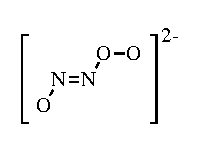
\includegraphics{picture/beta-N2O32-.eps}
        \end{minipage}
    }
    \caption{\ce{N2O3^2-}的两种异构体及其结构}
\end{figure}
\indent 另外,\ce{N2O2^2-}还可以作为配体.例如在\ce{[Co(NH3)5(NO)]^2+}的异构体\ce{[Co2(NH3)10(N2O2)]^4+}中就存在\ce{N2O2^2-}作为桥连配体,其结构如下:
\chemfig{Co2N2O2}{1}{\ce{[Co2(NH3)10(N2O2)]^4+}的结构}
在\ce{Pt(PPh3)2(N2O2)}中也存在\ce{N2O2^2-},其中两个\ce{O}原子对\ce{Pt}配位,形成螯合的五元环:
\chemfig{PtN2O2}{1}{\ce{Pt(PPh3)2(N2O2)}的结构}
\subsubsection{亚硝酸\ce{HNO2}及其盐}
\begin{substance}[\ce{HNO2}]
    亚硝酸,化学式为\ce{HNO2}.未分离出纯的\ce{HNO2}.
\end{substance}
\begin{substance}[\ce{NaNO2}]
    亚硝酸钠,俗称硝精,化学式为\ce{NaNO2},为淡黄色至无色的晶体,熔点为$284\tc$,沸点为$320\tc$.
\end{substance}
\paragraph{\ce{HNO2}及其盐的制备}
虽然没有分离出纯的\ce{HNO2},但它在气相中与\ce{H2O},\ce{NO}和\ce{NO2}存在如下平衡:
\begin{center}
    \ce{2HNO2(g) <=> H2O(g) + NO(g) + NO2(g)}\ \ \ $K=8.0\times10^5$
\end{center}
亚硝酸盐则可以通过对硝酸盐的部分还原而得到:
\begin{center}
    \ce{NaNO3 + Pb -> NaNO2 + PbO}
\end{center}
工业上采用\ce{NaOH}或\ce{Na2CO3}溶液吸收\ce{NO}和\ce{NO2}的混合物以制备\ce{NaNO2}:
\begin{center}
    \ce{Na2CO3 + NO + NO2 -> 2NaNO2 + CO2}
\end{center}
然后采用复分解反应制备其它亚硝酸盐;也可以通过复分解反应制备\ce{HNO2},例如:
\begin{center}
    \ce{Ba(NO2)2 + H2SO4 -> BaSO4 v + 2HNO2}
\end{center}
\paragraph{\ce{HNO2}及其盐的性质与应用}
\ce{HNO2}在水溶液中不稳定,可以按照下面的方式歧化分解:
\begin{center}
    \ce{3HNO2(aq) <=> H3O+(aq) + NO3-(aq) + 2NO(g)}
\end{center}
在强氧化剂的存在下,\ce{NO2-}可以被氧化为\ce{NO3-},例如可以用\ce{KMnO4}滴定\ce{NO2-}:
\begin{center}
    \ce{5NO2- + 2MnO4- + 6H+ -> 5NO3- + 2Mn^2+ + 3H2O}
\end{center}
亚硝酸盐本身也有一定氧化性.从天然盐卤提取碘单质的过程中,可以利用\ce{NaNO2}在酸性环境下与盐卤水反应:
\begin{center}
    \ce{2I- + 2NO2- + 4H+ -> I2 + 2NO + 2H2O}
\end{center}
前面已经提到过\ce{HNO2}可以与\ce{N2H5+}反应生成\ce{HN3}.后者可以与\ce{HNO2}进一步反应生成\ce{N2}与\ce{N2O}:
\begin{center}
    \ce{H\tbf{N}O2 + HN3 -> N2 + \tbf{N}NO + H2O}
\end{center}
\indent \ce{NaNO2}有低毒性.它经常被用于处理肉类,用于防腐和增色增香.因此,要警惕食用\ce{NaNO2}含量过高的腌制肉类.\\
\indent \ce{NaNO2}在有机化学中可用于对芳香胺进行重氮化反应:
\begin{center}
    \ce{ArNH2 + NaNO2 + 2HCl -> [Ar-N#N]Cl + NaCl + 2H2O}
\end{center}
\paragraph{\ce{NO2-}的配合物}
有关于\ce{NO2-}的配合物的最重要的性质是它形成的键合异构体,即以\ce{N}配位的硝基配合物和以\ce{O}配位的亚硝酸酯配合物.一般而言,硝基配位的形式更加稳定.典型的是下面两种化合物:黄色的\ce{[Co(NH3)5(NO2)]^2+}和红色的\ce{[Co(NH3)5(ONO)]^2+}.

\subsubsection{硝酸\ce{HNO3}及其盐}
\begin{substance}[\ce{HNO3}]
    硝酸,化学式为\ce{HNO3},是无色液体,熔点$-41.6\tc$,沸点$82.6\tc$.
\end{substance}
\paragraph{\ce{HNO3}的生产与用途}
1900年以前,大规模生产\ce{HNO3}完全依赖于以下复分解反应:
\begin{center}
    \ce{2NaNO3 + H2SO4 -> Na2SO4 + 2HNO3}
\end{center}
1903年,人们发明了电弧炉中直接制取\ce{HNO3}的方法:
\begin{center}
    \ce{2N2(g) + 5O2(g) + 2H2O(l) ->T[放电] 4HNO3(l)}
\end{center}
这一方法仍然需要消耗极高的能量以提供反应的活化能\footnote{从另一个角度而言,如果该反应的活化能较低,那么大气中将不再有\ce{O2},海洋中也将充满\ce{HNO3}.},因而十分昂贵.直到人们发明了\ce{NH3}的催化氧化:
\begin{center}
    \ce{2NH3 + 5O2 ->T[\ce{Pt}] 2NO + 3H2O}\\
    \ce{2NO + O2 -> 2NO2}\\
    \ce{3NO2 + H2O -> 2HNO3 + NO}
\end{center}

\indent 硝酸在工业中有非常重要而广泛的应用.
\paragraph{无水\ce{HNO3}的性质}
无水\ce{HNO3}中发生明显的离解反应:
\begin{center}
    \ce{2HNO3 <=> H2NO3+ + NO3-}\\
    \ce{H2NO3+ <=> NO2+ + H2O}\\
    \ce{H2O + HNO3 <=> H3O+ + NO3-}
\end{center}
这导致了无水\ce{HNO3}的\ce{^15N}NMR信号中只有一个\ce{HNO3},\ce{NO2+}和\ce{NO3-}平衡混合物的混合峰.
\paragraph{硝酸盐的热分解}
硝酸盐的热分解产物主要和金属元素有关.下面是一些例子.
\begin{center}
    \ce{2NaNO3 ->T[$\Delta$] 2NaNO2 + O2}\\
    \ce{4KNO3 ->T[$\Delta$] 2K2O + 2N2 + 5O2}\\
    \ce{2Pb(NO3)2 ->T[$\Delta$] 2PbO + 4NO2 + O2}\\
    \ce{2AgNO3 ->T[$\Delta$] Ag + 2NO2 + O2}
\end{center}
稍特殊一些的是硝酸铵\ce{NH4NO3}的分解.在高温下或使用引爆剂时,\ce{NH4NO3}发生爆炸性的分解;缓慢加热时则分解生成\ce{N2O}:
\begin{center}
    \ce{2NH4NO3 ->T[$>300\tc$] 2N2 + O2 + 4H2O}\\
    \ce{NH4NO3 ->T[$200\sim260\tc$] N2O + 2H2O}
\end{center}
\paragraph{\ce{NO3-}的配合物}
大部分\ce{NO3-}的配合物中\ce{NO3-}都作为双齿配体存在,当然也有少部分例外.
\paragraph{原硝酸根\ce{NO4^3-}}
尽管不存在\ce{H3PO4}的类似物\ce{H3NO4},原硝酸根\ce{NO4^3-}的盐却是已经制得的:
\begin{center}
    \ce{NaNO3 + Na2O ->T[$300\tc$][7 days] Na3NO4}
\end{center}
其中\ce{NO4^3-}的键长异常的小.这可能是\ce{N}与\ce{O}之间显著的电荷相互作用所致.
\end{document}